\section{Dinámica de los instrumentos indicadores}

Un instrumento analógico se compone de dos partes: una fija (estator) y una móvil (rotor). 
El principio es físico es simple: una fuerza (dependiente de la magnitud eléctrica a medir) empuja al rotor, produciendo un giro. A la relación entre lo que medimos y cuánto gira la aguja se le llama \emph{ley del instrumento}.

Resumen de los principales tipos de instrumentos y sus leyes de respuesta:

\begin{description}
  \item \textbf{Imán permanente y bobina móvil (PMMC)}
    \begin{itemize}
      \item \textit{Mide:} Corriente y tensión en \textbf{C.C.}
      \item \textit{Ley:} Lineal (\(\theta = K \cdot i\)).
    \end{itemize}
  \item \textbf{Hierro móvil}
    \begin{itemize}
      \item \textit{Mide:} Corriente y tensión en \textbf{C.C. y C.A.}
      \item \textit{Ley:} Cuadrática (\(\theta = \frac{dL}{d\theta}I^2\)).
    \end{itemize}
  \item \textbf{Electrodinámico}
    \begin{itemize}
      \item \textit{Mide:} Pohencia, corriente, tensión.
      \item \textit{Ley:} Depende del coseno de fase (\(\theta = \frac{dM}{d\theta}I_fI_m \cos(\beta)\)).
    \end{itemize}
  \item \textbf{Inducción}
    \begin{itemize}
      \item \textit{Mide:} Energía (medidores de luz) y potencia en \textbf{C.A.}
      \item \textit{Ley:} Depende del seno (\(\theta = K I_1 I_2 \sin(\beta)\)).
    \end{itemize}
\end{description}

\subsection{Ecuación general del movimiento (Las Cuplas)}

Para entender la dinámica, definiremos las fuerzas de rotación (Torques) como \textbf{Cuplas}. Para que la aguja se detenga en el valor correcto, deben interactuar tres tipos de cuplas:

\begin{enumerate}
    \item \textbf{Cupla Motora (\(C_m\)):} Es la fuerza que quiere mover la aguja. Su origen es eléctrico (magnético, electrostático, etc.).
    \item \textbf{Cupla Antagónica o Directriz (\(C_d\)):} Es la fuerza que ``tira hacia atrás''. Generalmente es un resorte que se retuerce. Si no existiera, la aguja daría vueltas completas como un motor.
    \item \textbf{Cupla de Amortiguamiento (\(C_a\)):} Es el freno. Solo aparece cuando hay movimiento y evita que la aguja oscile eternamente alrededor del valor final.
\end{enumerate}

La ecuación diferencial que describe el equilibrio dinámico es:
\[ C_m = C_d + C_a + C_i \]
Donde \(C_i\) es la inercia del sistema (\(J \frac{d^2\theta}{dt^2}\)).

\subsection[Análisis de la Cupla Directriz]{Análisis de la Cupla Directriz (\(C_d\))}

La cupla directriz (o de restitución) suele generarse mediante resortes en espiral o cintas de torsión. Su fuerza es proporcional al ángulo girado (Ley de Hooke angular):
\[ C_d = K_r \cdot \theta \]
Donde \(K_r\) depende del material (bronce-fosforoso) y la geometría del resorte.

\subsubsection{El proceso de equilibrio}
Imaginemos que conectamos el instrumento. La aguja empieza en cero:
\begin{enumerate}
    \item Al principio, la \textbf{Cupla Motora} es máxima y la \textbf{Antagónica} es cero. La aguja acelera.
    \item A medida que la aguja gira (\(\theta\) crece), el resorte se tensa y la Cupla Antagónica aumenta, oponiéndose al movimiento.
    \item El equilibrio se alcanza teóricamente cuando ambas fuerzas se igualan: \(C_m = C_d\).
\end{enumerate}

El gráfico de la figura \ref{fig_cuplas_instrumentales} ilustra cómo la Cupla Directriz (\(C_d\), línea roja) crece linealmente hasta cruzar las líneas de Cupla Motora (\(C_{m1}, C_{m2}\)), determinando los ángulos de equilibrio \(\theta_1\) y \(\theta_2\).

\begin{figure}[ht]
  \centering
  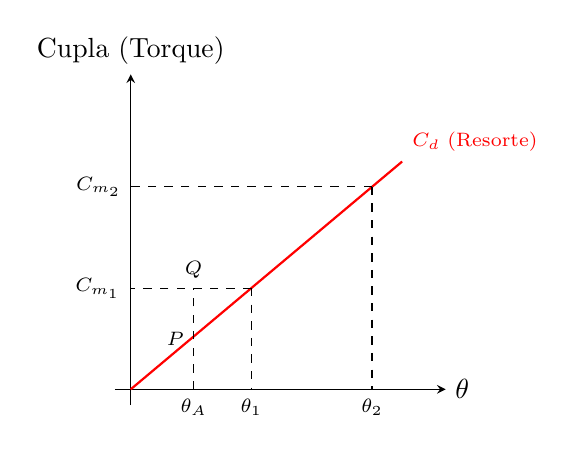
\begin{tikzpicture}[>=stealth]
    % Axis
    \draw[->] (-0.2,0) -- (4,0) node[right] {\(\theta\)};
    \draw[->] (0,-0.2) -- (0,4) node[above] {Cupla (Torque)};

    % cd curve (Linear Spring)
    \draw[red,thick] (0,0) -- (40:4.5) node[above right] {\scriptsize{\(C_d\) (Resorte)}};

    % intersections to cd (Equilibrium points)
    \draw[dashed] (40:2) -- ++(-1.54,0) node[left] {\scriptsize{\(C_{m_1}\)}};
    \draw[dashed] (40:4) -- ++(-3.06,0) node[left] {\scriptsize{\(C_{m_2}\)}};
    
    % Dropping lines to alpha axis
    \draw[dashed] (40:2) -- ++(0,-1.29) node[below] {\scriptsize{\(\theta_1\)}};
    \draw[dashed] (40:4) -- ++(0,-2.57) node[below] {\scriptsize{\(\theta_2\)}};
    
    % Visualizing the forces
    \draw[dashed] (0.8,0) node[below]{\scriptsize{\(\theta_A\)}} -- node[left]{\scriptsize{\(P\)}} (0.8,1.29) node[above]{\scriptsize{\(Q\)}};
  \end{tikzpicture}
  \caption{Interacción entre Cupla Motora (horizontal) y Directriz (diagonal). El punto de cruce es la lectura final.}
  \label{fig_cuplas_instrumentales}
\end{figure}

\subsection[Cuplas de amortiguamiento]{Cuplas de Amortiguamiento (\(C_a\))}

Esta cupla es necesaria para disipar la energía cinética. Sin ella, la aguja oscilaría mucho tiempo antes de detenerse. Existen tres tipos principales:

\subsubsection{1. Amortiguamiento por Rozamiento Sólido (Indeseable)}
Es el roce entre el eje y los pivotes. \textbf{Es malo} porque introduce un error: la aguja se detiene un poco antes o un poco después del valor real (zona de incertidumbre \(\delta\)).

\subsubsection{2. Amortiguamiento Fluido (Por aire)}
Se usa un aspa moviéndose dentro de una cámara cerrada (como un pistón de aire). Es común en instrumentos de Hierro Móvil.

\subsubsection{3. Amortiguamiento Magnético (Frenado por Corrientes de Foucault)}
Es el más efectivo y elegante. Se basa en la Ley de Lenz: \emph{``El movimiento induce una corriente que se opone a la causa que lo produce''}.

\textbf{¿Cómo funciona paso a paso?} 
\begin{enumerate}
    \item Un disco (o bobina) de aluminio conductor se mueve a velocidad \(v\) dentro de un campo magnético \(B\).
    \item Se induce una fuerza electromotriz (f.e.m.): \( e = B \cdot l \cdot v \).
    \item Como el material es conductor, circula una corriente: \( i = e / R \).
    \item Esta corriente interactúa con el imán creando una fuerza de frenado: \( F = B \cdot l \cdot i \).
\end{enumerate}

Sustituyendo las ecuaciones, obtenemos que el torque de frenado es proporcional a la velocidad angular \(\omega\):
\[ C_a = \left( \frac{B^2 l^2 r^2}{R} \right) \cdot \omega = D \cdot \omega \]
Donde \(D\) es la constante de amortiguamiento. Para que frene bien, necesitamos baja resistencia \(R\) (por eso usamos aluminio) y un campo magnético \(B\) fuerte.

\textbf{Caso especial: Bobina Móvil}
En los instrumentos de bobina móvil, la propia bobina actúa como freno si el circuito externo es de baja resistencia. Además, la bobina suele enrollarse sobre un marco de aluminio. El frenado total es la suma de dos efectos:
\[ D_{\text{total}} = D_{\text{bobina}} + D_{\text{marco aluminio}} \]
\[ D = B^2 l^2 a^2 \left( \underbrace{\frac{N^2}{R}}_{\text{Circuito}} + \underbrace{\frac{S_{Al}}{2\rho(l+a)}}_{\text{Marco de Al}} \right) \]

Todos estos sistemas de amortiguamiento, y cuplas se encuentran materializados en el instrumento como se muestra en la figura \ref{fig_galvanometro}, que ilustra un galvanómetro de imán permanente y bobina móvil.

\begin{figure}[ht]
  \centering
  \includegraphics[width=0.5\textwidth]{chapters/1_unit/media/bin/galvanometro.pdf}
  \caption{Galvanómetro de imán permanente y bobina móvil.}
  \label{fig_galvanometro}
\end{figure}

\subsection{Sistemas de Suspensión}
Para minimizar el error por rozamiento sólido, se utilizan pivotes de alta calidad (piedras preciosas) o, en instrumentos de alta precisión, suspensión por \textbf{cinta tensa}, que elimina totalmente la fricción mecánica al hacer flotar el sistema móvil .

\section{Estudio de la ecuación del movimiento}

\subsection{Ecuación del movimiento de un sistema móvil alrededor de un eje}

El estudio de la ecuación del movimiento en un instrumento eléctrico indicador, conduce a la obtención de la respuesta del mismo relacionada con los distintos parámetros que lo constituyen en función del tiempo. 

Por la simplicidad y conveniencia de su diseño eléctrico y mecánico, el movimiento del sistema indicador de un instrumento eléctrico es generalmente un movimiento de rotación. Se puede considerar que estos dispositivos mecánicos tienen un solo grado de libertad: el de rotación alrededor de su eje. La ecuación mecánica a plantear es la que determina que la suma de los pares actuantes sobre un cuerpo rígido con un solo grado de libertad, es igual a la variación del momento angular del sistema móvil
\[
  \sum_{k=1}^n C_k = \frac{d\bar{H}}{dt}
\]
el vector \(H\), tiene una sola componente a lo largo del eje de rotación, por lo que su expresión se reduce: donde \(J\) es el momento de inercia del sistema móvil y \(\theta\) es la posición angular instantánea del sistema móvil.
\[
  \sum{k=1}^n c_k = J\frac{d^2\theta}{dt^2} = J\gamma = C_i
\]
Es decir que la sumatoria de las cuplas actuantes iguala a la cupla de inercia:
\begin{gather*}
  H=J\frac{d\theta}{dt} \\ 
  C_m - C_a - C_d \pm C_r = C_i
\end{gather*}
Reemplazando por sus respectivas expresiones y ordenando términos se tendrá:
\[
  J\frac{d^2\theta}{dt^2} + D\frac{d\theta}{dt} + K\theta \pm C_r = C_m
\]
Suponiendo despreciable al rozamiento:
\[
  C_m = J\frac{d^2\theta}{dt^2} + D\frac{d\theta}{dt} + K\theta
\]
que resulta la ecuación diferencial del movimiento de un instrumento.

Es decir que la cupla motora iguala a la suma de las cuplas de inercia, de amorguamiento y del resorte.

\subsection{Solución de la ecuación diferencial}

Es fundamental tener noción básica (o superficial) de ecuaciones diferenciales y funciones de variable compleja para comprender este apartado. En el libro \citetitle{c4elio} de \textcite{c4elio} se presentan las funciones de variable compleja en los primeros capítulos.

Las ecuaciones diferenciales lineales de segundo orden en coeficientes constantes, se encuentran a menudo en los estudios técnicos. Un ejemplo ya conocido en teoría de circuitos lo representa la corriente de malla del circuito serie RLC.

Para resolver la ecuación del movimiento del instrumento de rotación, podemos determinar que \(\theta=f_t\). Esta función es importante ya que nos permitirá determinar en qué forma se produce el movimiento en los instrumentos de rotación en función del tiempo.

La solución general de una EDO lineal con coeficientes constantes consiste en la suma de una solución particular \(\theta_p\) (que representa el estado permanente o estacionario final e independiente del tiempo) y una solución homogénea \(\theta_h\) (representativa del estado transitorio), que tiende a desaparecer con el tiempo.
\[
  \theta = \theta_p + \theta_h
\]

La solución general debe tener las constantes arbitrarias que indique el orden de la ecuación diferencial (en nuestro caso dos, ya que es de segundo orden). Para hallar la solución homogénea se plantea la ecuación homogénea:
\begin{equation}\label{eq:edo_instrumento}
  J\frac{d^2\theta}{dt^2} + D\frac{d\theta}{dt} + K\theta = J\ddot{\theta} + D\dot{\theta} + K\theta = 0
\end{equation}

\begin{tcolorbox}[title=Recordatorio]
  La notación \(\ddot{\theta}\) es conocida como la notación de Newton para las derivadas. Así, \(\ddot{\theta}=\theta''\) y, de la misma manera \(\dot{\theta}=\theta'\).
  % He colocado esta nota según mis conocimientos. Dime si esto es incorrecto.
\end{tcolorbox}

Entonces, propone la solución de la EDO homogénea,
\[
  \theta_h = Ae^{rt}
\]
siendo \[A\] una constante arbitraria y \(r\) una constante a determinar.
\[
  \dot{\theta} = Are^{rt} \qquad \text{y} \quad \ddot{\theta} = Ar^2e^{rt}
\]
Reemplazando en la ecuación \eqref{eq:edo_instrumento} con la solución homogénea,
\begin{equation}\label{eq:solucion_de_edo}
  Ae^{rt}(Jr^2+Dr+K) = 0
\end{equation}
Para encontrar los valores de \(r\) para los cuales la ecuación \eqref{eq:solucion_de_edo} se cumple, entonces:
\[
  Jr^2 + Dr + K = 0
\]
ya que \(A\neq0\) y \(e^{rt}\) no puede ser cero. Así, 
\begin{align}\label{eq_solucion_caracteristica_1}
  r_1 &= -\frac{D}{2J} + \sqrt{\frac{D^2}{4J^2}-\frac{K}{J}} \\ \label{eq_solucion_caracteristica_2}
  r_1 &= -\frac{D}{2J} - \sqrt{\frac{D^2}{4J^2}-\frac{K}{J}}
\end{align}
y entonces la solución del régimen libre estará formada por dos términos:
\[
  \boxed{\theta_h=Ae^{r_1t}+Be^{r_2t}}
\]
Siendo \(B\) otra constante arbitraria y \(r_1\) distinta de \(r_2\).

La solución particular \(\theta_p\) en el régimen permanente o estacionario se encuentra haciendo \(\theta_p=E=\text{constante}\), y reemplazando en la ecuación diferencial. Así, 
\[
  K\theta_p=C_m
\]
Luego la solución general será:
\[
  \theta = \theta_p + \theta_h = \frac{C_m}{K}+Ae^{r_1t}+Be^{r_2t}
\]
donde \(r_1\) y \(r_2\) son las soluciones \eqref{eq_solucion_caracteristica_1} y \eqref{eq_solucion_caracteristica_2} de la ecuación característica. Por tanto \(A\) y \(B\) dependen de las condiciones iniciales.

Podemos establecer que para \(t=0\),
\[
  \theta_i = 0 \qquad \text{y}\qquad \frac{d\theta}{dt}=0
\]
Así, calculamos \(A\) y \(B\). Para la primera condición:
\begin{equation}\label{eq_theta}
  \theta=\theta_p + Ae^{r_1\theta}+Be^{r_2\theta}
\end{equation}
Para la segunda, calcule la derivada e iguale a cero:
\begin{equation}\label{eq_theta_derivada}
  \frac{d\theta}{dt}=0 + r_1Ae^{r_1 0}+r_2Be^{r_2 0}
\end{equation}
De \eqref{eq_theta} y \eqref{eq_theta_derivada} obtenemos:
\begin{align*}
  A &= -\frac{r_2}{r_2-r_1}\theta_p \\ 
  B &= -\frac{r_1}{r_2-r_1}\theta_p
\end{align*}
Entonces, reemplazando \(A\) y \(B\) en \eqref{eq_theta}
\[
  \theta = \theta_p (1-\frac{r_2}{r_2-r_1}e^{r_1t}-\frac{r_1}{r_2-r_1 e^{r_2t}})
\]
Analicemos ahora los valores que pueden tomar las raíces de la ecuación característica (ecuaciones \eqref{eq_solucion_caracteristica_1} y \eqref{eq_solucion_caracteristica_2}).
\begin{enumerate}
  \item Movimiento Periódico: Si 
    \[
      \frac{D^2}{4J^2} < \frac{K}{J}
    \]
    tendremos raíces complejas conjugadas,
    \begin{align*}
      r_1 &= -\frac{D}{2J}+j\sqrt{\frac{K}{J}-\frac{D^2}{4J^2}} \\ 
      r_2 &= -\frac{D}{2J}-j\sqrt{\frac{K}{J}-\frac{D^2}{4J^2}} 
    \end{align*}
    que al reemplazar estas soluciones en la expresión de \(\theta\) y operar algebráicamente, se puede obtener que
    \[
      \theta = \theta_p \left[1+e^{-at}\left(-\frac{a}{b}\cdot \frac{e^{jbt}-e^{-jbt}}{2j}\right)+\left(\frac{e^{jbt}+e^{-jbt}}{2}\right)\right]
    \]
    De tal forma que se pueden usar las relaciones de Euler,
    \[
      \theta = \theta_p \left[a \sin(bt)+ b\cos(bt)\right]
    \]
    Esta expresión presenta una función armónica de amplitud decreciente con el tiempo, y pulsación mecánica de valor \(b\).

    Este es el caso oscilatorio o subamortiguado y desde el punto de vista práctico es el de mayor utilidad. En los instrumentos se requiere para llegar a la posición permanente un movimiento \emph{ligeramente subamortiguado}.
    % Se debe realizar un gráfico de \theta/\theta_p
  \item Movimiento crítico:
  \item Movimiento aperiódico: 
\end{enumerate}

\subsection{Respuesta a una excitación sinusoidal}
